\section{实验结果与分析}
\subsection{五折模型比较}
表\ref{tab:cv}与图\ref{fig:cv}给出六类模型的训练集开发结果。逻辑回归的宏平均 F1 为 0.9339，融合模型为 0.9318，二者均值差为 0.0021，远小于各自约 0.04 的折间标准差。单次基础种子 42 下，融合比 MLP 和 CNN 的均值分别高约 0.0032 和 0.0077；这些差异尚不能证明显著提升。
\begin{table}[htbp]\centering\small
\caption{六类模型的五折分组开发结果}\label{tab:cv}
\begin{tabular}{lrrr}\toprule
模型 & 训练 F1 均值 & 验证 F1 均值 & 折间标准差\\\midrule
逻辑回归 & 0.9934 & 0.9339 & 0.0427\\
SVM & 0.9962 & 0.9292 & 0.0389\\
随机森林 & 0.9999 & 0.9165 & 0.0453\\
MLP & 0.9939 & 0.9286 & 0.0427\\
1D CNN & 0.9656 & 0.9241 & 0.0438\\
融合模型 & 0.9807 & 0.9318 & 0.0438\\
\bottomrule\end{tabular}
\tabnote{F1 均为宏平均；神经网络基础种子为 42。传统模型在同一组折上搜索参数，分数存在选择乐观性。}
\end{table}

\begin{figure}[htbp]\centering
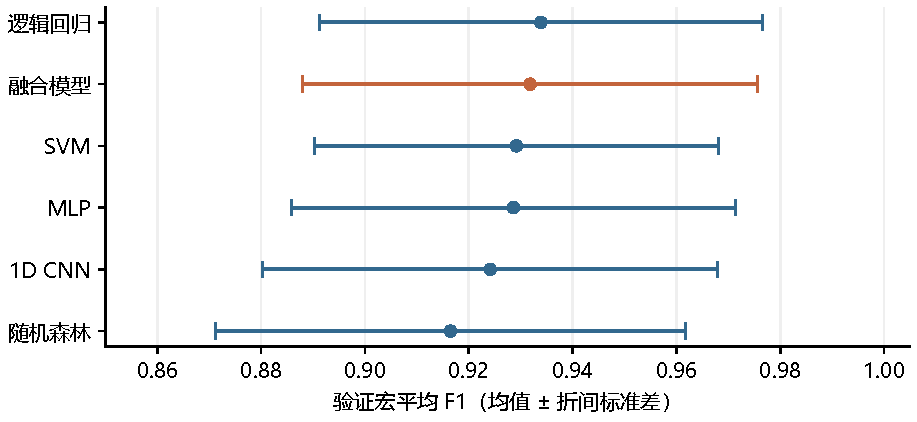
\includegraphics[width=.88\linewidth]{cv_comparison.pdf}
\caption{训练集五折分组交叉验证的宏平均 F1。误差线为折间标准差（ddof=0），不是置信区间；神经网络使用基础种子 42。}\label{fig:cv}
\end{figure}

逻辑回归、MLP 与融合模型的训练 F1 均明显高于验证 F1，反映了拟合训练窗口与识别新受试者之间的差距；随机森林训练 F1 接近 1，验证均值却最低。模型容量增加没有保证跨受试者性能同步提升。融合网络在第 1、2 折的验证 F1 分别约为 0.8910、0.9013，在第 3、4 折则约为 0.9900、0.9804，说明不同验证受试者组合与显著不同的难度相伴随，但现有实验不足以分离体态、动作习惯或采集条件各自的影响。

\subsection{正则化与 PCA 对照}
逻辑回归在 $C=0.001$ 时的验证宏平均 F1 为 0.9130，$C=0.1$ 时达到 0.9339，增至 $C=10$ 后降至 0.9280，而训练 F1 上升至约 0.9998。这说明在本次搜索范围内，适中的正则化取得了较好折中。RBF SVM 在 $\gamma=0.01$ 时训练 F1 接近 1，验证 F1 约为 0.84，也呈现明显的训练与验证差距。
\begin{table}[htbp]\centering\small
\caption{固定逻辑回归 $C=0.1$ 的 PCA 对照}\label{tab:pca}
\begin{tabular}{lrrrr}\toprule
设置 & 各折维数范围 & 验证 F1 & 折间标准差 & 耗时/s\\\midrule
不使用 PCA & 561 & 0.9339 & 0.0427 & 218.9\\
PCA 90\% & 62 & 0.9036 & 0.0537 & 83.9\\
PCA 95\% & 100--101 & 0.9205 & 0.0455 & 56.4\\
PCA 99\% & 177--178 & 0.9280 & 0.0443 & 262.6\\
\bottomrule\end{tabular}
\tabnote{保留比例指累计解释方差；各设置未重新搜索分类器参数，耗时为本机单次五折运行记录。}
\end{table}


表\ref{tab:pca}中，保留 95\% 方差将维数减少至约 100，但验证 F1 降至 0.9205；保留 99\% 方差时为 0.9280，仍低于不降维结果。可能的解释是，较低方差的方向中仍含有分类所需信息。不过，本实验对各 PCA 设置固定 $C=0.1$，未分别重新调参，因此只能评价当前组合，不能证明 PCA 对该任务普遍无效。95\% 设置的单次运行耗时较短，但 99\% 设置反而更慢，提示求解迭代与系统状态也会影响耗时。

\subsection{融合模型的随机性复验}
\begin{table}[htbp]\centering\small
\caption{融合模型三个基础种子的分组验证结果}\label{tab:seeds}
\begin{tabular}{lrrl}\toprule
基础种子 & 五折平均 F1 & 折间标准差 & 各折选定轮数\\\midrule
42 & 0.9318 & 0.0438 & 11, 9, 16, 3, 1\\
2024 & 0.9330 & 0.0433 & 9, 11, 29, 10, 6\\
2025 & 0.9295 & 0.0374 & 6, 11, 17, 3, 1\\
\bottomrule\end{tabular}
\tabnote{三次五折均值平均为 0.9314，均值间样本标准差（ddof=1）为 0.0018；外层与内层受试者划分均固定。}
\end{table}

三个基础种子对应的五折均值平均为 0.9314，均值之间的样本标准差为 0.0018，低于各次运行约 0.0374--0.0438 的折间标准差。这表明在固定受试者划分下，所观察的初始化及批次随机性波动小于受试者组合间的分数波动；它不等价于对任意受试者划分都稳定。部分内层选择轮数仅为 1 或 3，也提示早停对特定内层受试者组合较敏感。由于 MLP 与 CNN 未做相同次数的多种子复验，这里不将融合相对于单分支的差值解释为稳健优势。

\subsection{官方独立测试与类别误差}
\begin{table}[htbp]\centering\small
\caption{冻结模型的官方独立测试结果}\label{tab:test}
\begin{tabular}{lrrr}\toprule
模型 & 准确率 & 宏平均 F1 & 错误窗口数\\\midrule
逻辑回归 & 0.9498 & 0.9500 & 148\\
融合模型 & 0.9555 & 0.9564 & 131\\
\bottomrule\end{tabular}
\tabnote{共 2947 个窗口、9 名受试者。两模型配置均在独立测试前固定。}
\end{table}

冻结后的测试结果见表\ref{tab:test}。融合的准确率比逻辑回归高 0.58 个百分点，宏平均 F1 高 0.64 个百分点，错误数从 148 减至 131。交叉验证均值与独立测试的相对排序不同，说明两种评价所涉及的受试者组合可能影响结论；不能使用测试结果回头改变此前的模型选择规则。

逐样本配对比较显示，两模型共同识别正确 2754 个窗口，共同出错 86 个；融合修正了逻辑回归的 62 个错误，同时新增了 45 个逻辑回归原本识别正确的错误，净改善为 17 个。按测试受试者统计，融合的准确率在 6 人上提高、2 人上降低、1 人上相同；例如受试者 10 从 82.65\% 降至 77.55\%。因此，总体均值提升不能表述为每名受试者均受益。两个模型的混淆矩阵见图\ref{fig:cm-lr}、图\ref{fig:cm-fusion}，各类别 F1 见图\ref{fig:class}。
\begin{figure}[htbp]\centering
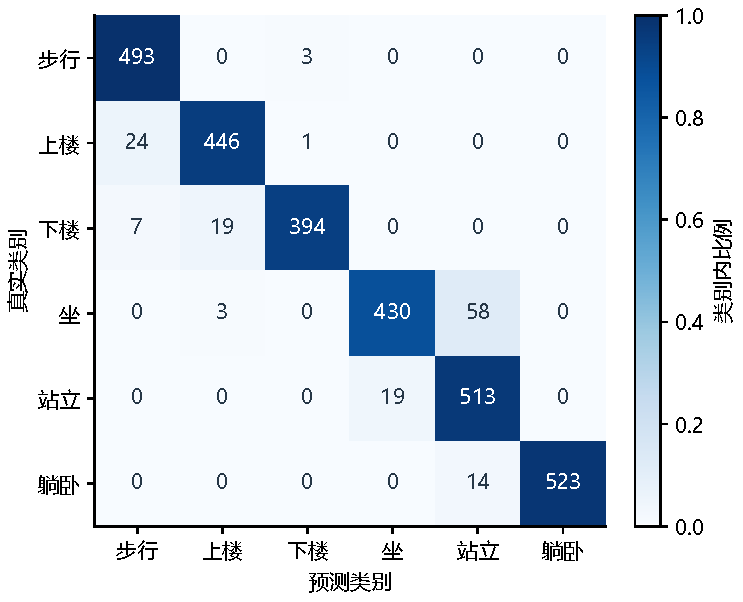
\includegraphics[width=.78\linewidth]{cm_logistic.pdf}
\caption{逻辑回归的独立测试混淆矩阵。行表示真实类别，列表示预测类别；数字为样本数，颜色按真实类别逐行归一化。}\label{fig:cm-lr}
\end{figure}
\begin{figure}[htbp]\centering
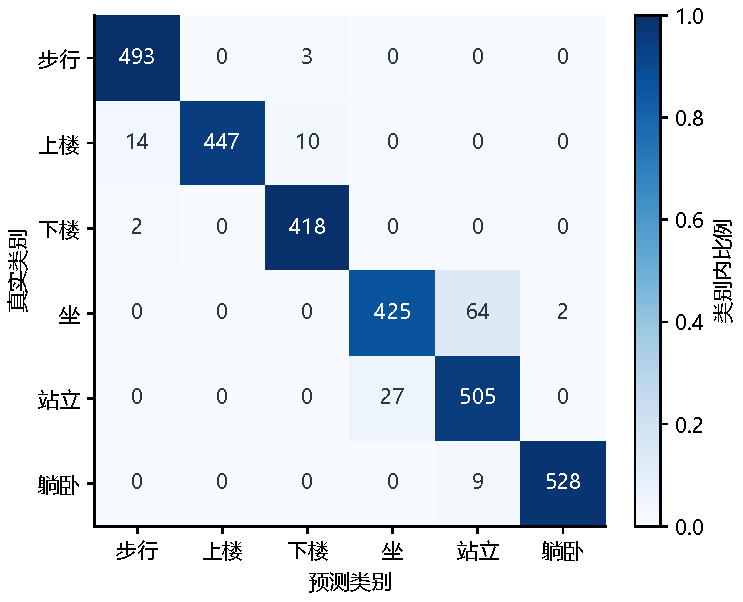
\includegraphics[width=.78\linewidth]{cm_fusion.pdf}
\caption{融合模型的独立测试混淆矩阵。与图\ref{fig:cm-lr}采用相同归一化方式和颜色范围。}\label{fig:cm-fusion}
\end{figure}
\begin{figure}[htbp]\centering
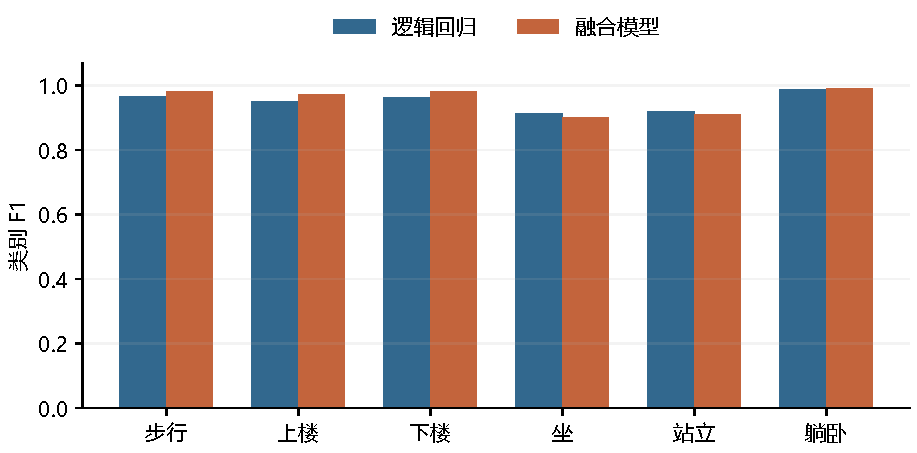
\includegraphics[width=.88\linewidth]{class_f1.pdf}
\caption{两冻结模型在独立测试集各类别上的 F1。融合在动态活动上提高，而坐与站立下降。}\label{fig:class}
\end{figure}

图\ref{fig:cm-lr}至图\ref{fig:class}揭示收益的不均衡。融合的步行、上楼和下楼 F1 分别为 0.9811、0.9739、0.9824，高于逻辑回归的 0.9667、0.9499、0.9633；躺卧略有提高。但坐与站立 F1 分别从 0.9149、0.9185 降至 0.9014、0.9099。融合将 64 个坐窗口误判为站立、27 个站立窗口误判为坐，这 91 个错误占其全部错误的 69.47\%。原始数据论文也讨论了坐与站立之间的混淆问题\cite{anguita2013}，但本实验没有姿态标注或传感器位置干预，不能进一步确证误差的物理原因。

\subsection{讨论与局限}
双分支学习在本次官方测试中提供了较好的总体结果，但没有在所有评价条件下超过强线性基准。人工统计特征已经编码大量活动信息，融合的额外容量可能带来互补信息，也可能放大对训练分布的适应。现有结果支持“当前配置存在局部收益”这一有限结论，而不支持原创架构、普遍优势或最先进性能的宣称。

实验仍有四方面限制。第一，传统模型在同一五折结果上调参与报告，神经网络则使用内层轮数选择，两者调参预算与选择方式不同；模型间比较不是完全对称的嵌套评估。第二，只有融合进行了三次训练随机性复验，且外层受试者划分固定。第三，官方测试仅含 9 人，相邻窗口共享采样点，窗口结果存在相关性，因此没有按独立同分布窗口作显著性检验，也未将折间标准差解释为泛化置信区间。第四，数据来自受控场景与固定设备，不能直接代表日常自由活动、其他佩戴位置或新设备下的表现。

进一步研究可在保留新的独立评价数据的前提下，统一嵌套调参预算、对单分支同样开展多种子及多受试者划分复验，并针对坐与站立引入可验证的姿态信息或融合约束。当前官方测试已用于结果分析，不能再据其反复调参后仍称为未触碰的最终测试。
